\chapter{Introduction}

The Roa Logic AHB-Lite PLIC (Platform Level Interrupt Controller) IP is a fully parameterised soft IP implementing the Interrupt Controller defined in the \emph{\href{https://github.com/riscv/riscv-isa-manual/blob/master/release/riscv-privileged-v1.9.1.pdf}{RISC-V Privileged v1.9.1 specification}}\footnote{Full specification details are provided in the References section}.

The IP features an AHB-Lite Slave interface, fully compliant with the \emph{\href{https://www.arm.com/products/system-ip/amba-specifications}{AMBA 3 AHB-Lite v1.0}} specifications. 

Bus address and data widths as well as the number of Interrupt Sources and Targets supported are configurable via compile-time parameters. The controller further supports user configurable priority levels and pending events, in addition to interrupt masking via programmable priority thresholds.

\begin{figure}[!htb]
  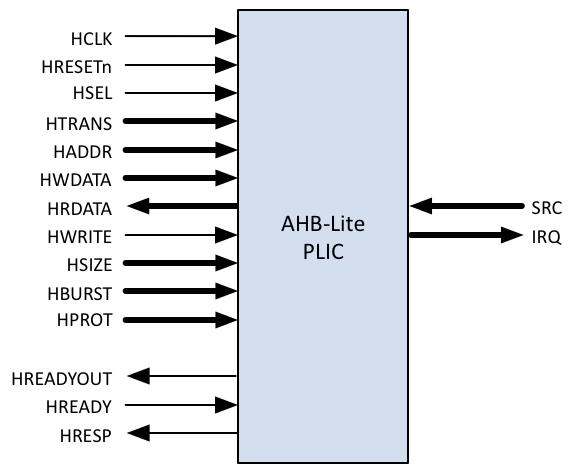
\includegraphics{assets/img/plic-ports}
  \caption{PLIC Port Diagram}
  \label{fig:PORTDIAG}
\end{figure}

\section{Features}

\begin{itemize}
	\item
		AHB-Lite Interface with parameterised address and data width
	\item
		User defined number of Interrupt Sources and Targets
	\item
		User defined priority level per Interrupt Source
	\item
		Interrupt masking per target via Priority Threshold support
	\item
		User defined Interrupt Pending queue depth per source
\end{itemize}
